\documentclass{article}
\usepackage{neurips_2019}

\usepackage[utf8]{inputenc} % allow utf-8 input
\usepackage[T1]{fontenc}    % use 8-bit T1 fonts
\usepackage{hyperref}       % hyperlinks
\usepackage{url}            % simple URL typesetting
\usepackage{booktabs}       % professional-quality tables
\usepackage{amsfonts}       % blackboard math symbols
\usepackage{nicefrac}       % compact symbols for 1/2, etc.
\usepackage{microtype}      % microtypography
\usepackage{graphicx}

% Useful packages
\usepackage{amsmath, amssymb, amsfonts, bm}
\usepackage{amsthm}
\usepackage{mathtools}
\usepackage[usenames, dvipsnames]{color}

\usepackage{enumitem}
%\setlist{leftmargin=*} 
%\setlist[enumerate]{label=\arabic*)}
%\setlist[enumerate, 1]{labelindent=20pt}


% \usepackage{blindtext}

\newtheorem{theorem}{Theorem}
\newtheorem{proposition}[theorem]{Proposition}
\newtheorem{corollary}[theorem]{Corollary}
\newtheorem{lemma}[theorem]{Lemma}
\newtheorem{remark}[theorem]{Remark}

\theoremstyle{remark}
\newtheorem*{notation}{Notation}
%\newtheorem*{remark}{Remark}
\newtheorem*{note}{Note}

\theoremstyle{definition}
\newtheorem{definition}[theorem]{Definition}
\newtheorem{fact}{Fact}
\newtheorem*{observation}{Observation}
\newtheorem*{condition}{Condition}
\newtheorem*{claim}{Claim}
\newtheorem*{example}{Example}
\newtheorem*{question}{Question}


\newcommand{\mypara}[1]{\paragraph{\fcolorbox{OliveGreen}{white}{\color{Violet}{#1}}}}

\newcommand{\tk}[1]{\textcolor{red}{TK: #1}}
\newcommand{\ao}[1]{\textcolor{green}{AO: #1}}
\newcommand{\tsj}[1]{\textcolor{magenta}{TSJ: #1}}
\newcommand{\va}[1]{\textcolor{blue}{Vincent A: #1}}

\newcommand{\Reals}{\mathbb{R}}
\newcommand{\T}{\mathsf{T}}
\DeclareMathOperator{\softmax}{\mathrm{softmax}}

\newcommand{\cA}{\mathcal{A}}
\newcommand{\cG}{\mathcal{G}}
\newcommand{\cK}{\mathcal{K}}
\newcommand{\cH}{\mathcal{H}}

\newcommand{\vect}[1]{\mathbf{#1}}
\newcommand{\vx}{\vect{x}}
\newcommand{\vy}{\vect{y}}
\newcommand{\vone}{\vect{1}}
\newcommand{\proj}{\mathrm{proj}}



\title{A New Model}

\author{}

\begin{document}

\maketitle

\section{VWM model}

\begin{notation}
Treat 1D tensors as column vectors and 2D tensors as matrices, where appropriate.
We use lower case to represent tensors but for matrix operations we will use upper case to 
refer to 2D tensors.

\begin{enumerate}
	\item  Let $\circ$ denote concatenation of two tensors with identical shape except possibly
	for their last dimensions $d_1$ and $d_2$, respectively,  
	resulting in a tensor with last dimension of $d_1+d_2$. 
	
	\item Let $\odot$ denote  element-wise product of two tensors of same shape,
	i.e., Hadamard product for vectors/matrices.
	
	\item Let $\otimes$ denote tensor product of two tensors, 
	i.e. Kronecker product for vectors/matrices.
\end{enumerate}
\end{notation}	

\section{Basic layers/modules}

\mypara{Linear (Affine) Layer}

\begin{description}
	\item[Inputs:] A tensor $x$ with last dimension $n$.
	\item[Parameter:] An affine function $\cG: \Reals^n \to \Reals^m$ with 
	weight and bias parameters.
		
	\item[Output:] A tensor $y$ with last dimension $m$, and remaining dimensions
	same as that of $x$, obtained by applying $\cG$ to each 1D slice of $x$
	along the last dimension.
	\end{description}

\hrulefill

\mypara{Attention Module}

\begin{description}
	\item[Inputs:] 
	\begin{enumerate}
		\item[]
		\item Query: $q \in \Reals^d$
		\item Keys: $K \in \Reals^{N \times d}$	
		\item Values: $V \in \Reals^{N \times d}$. By default $V=K$, unless mentioned explicitly.	
	\end{enumerate}

	\item[Parameter:] Weight $w \in \Reals^d$

	\item[Outputs:] 
	\begin{enumerate}
		\item[]
		\item Content vector: $h =  V^{\T} u \in \Reals^d$
		\item Attention vector:  $w = \softmax(K(w \odot q)) \in \Reals^N$
	\end{enumerate}
\end{description}

\hrulefill

\mypara{Interaction Module}

\begin{description}
	\item[Inputs:] 
	\begin{enumerate}
		\item[]
		\item Base object: $b \in \Reals^d$
		\item Feature objects: $f \in \Reals^{M \times d}$	
	\end{enumerate}
	
	\item[Parameters:] 
	\begin{enumerate}
	\item[]
	\item Base object projection linear layer: $\cG: \Reals^d \to \Reals^d$
	\item Feature objects projection linear layer : $\cK: \Reals^{M \times d} \to \Reals^{M \times d}$
	\item Modifier linear layer:  $\cH: \Reals^{M \times 2d} \to \Reals^{M \times d}$	
\end{enumerate}
		
	\item[Output:] Modified feature objects 
	$f' =  \cH( \cK(f) \odot ( \vone \otimes \cG(b))) \in  \Reals^{M \times d}$
\end{description}

\hrulefill

\section{VWM Cell}

\mypara{Question-driven Controller}

\begin{description}
	\item[Inputs:] 
	\begin{enumerate}
		\item[]
		\item Previous control state: $c \in \Reals^d$.	
		\item Reasoning step index $s$.
		\item Contextual words: $cw \in \Reals^{L \times d}$.
		\item Question encoding: $q \in \Reals^d$.
	\end{enumerate}
	
	\item[Parameters:] 
	\begin{enumerate}
		\item[]
		\item Position-aware linear layer: $\cG_s: \Reals^d \to \Reals^d$, depending on $s$.
		\item Concatenation layer: $\cH: \Reals^{2d} \to \Reals^d$.
		\item Attention module $\cA$.
		\item Temporal classifier:  $\cK: \Reals^d \to \Reals^4$. A two-layer feedforward
		network with ELU activation in the hidden layer of $d$ units.	
	\end{enumerate}
	
	\item[Outputs:] 
	\begin{enumerate}
		\item[]
		\item New control state $c'$.
		\item Control attention $ca$.
		\item Temporal class weights $\tau$.
    \end{enumerate}
	computed as follows:
\begin{enumerate}[label=\alph*.]
	\item Position-aware modulation $y = \cH([c, \cG_s(q)])$.
	\item Content and attention: $c', a = \cA(y, cw)$.
	\item Temporal classification: $\tau = \cK(c')$.
\end{enumerate}
\end{description}

\hrulefill

\mypara{Question-driven Controller}

\begin{description}
	\item[Inputs:] 
	\begin{enumerate}
		\item[]
		\item Previous control state: $c \in \Reals^d$.	
		\item Reasoning step index $s$.
		\item Contextual words: $cw \in \Reals^{L \times d}$.
		\item Question encoding: $q \in \Reals^d$.
	\end{enumerate}
	
	\item[Parameters:] 
	\begin{enumerate}
		\item[]
		\item Position-aware linear layer: $\cG_s: \Reals^d \to \Reals^d$, depending on $s$.
		\item Concatenation layer: $\cH: \Reals^{2d} \to \Reals^d$.
		\item Attention module $\cA$.
		\item Temporal classifier:  $\cK: \Reals^d \to \Reals^4$. A two-layer feedforward
		network with ELU activation in the hidden layer of $d$ units.	
	\end{enumerate}
	
	\item[Outputs:] 
	\begin{enumerate}
		\item[]
		\item New control state $c'$.
		\item Control attention $ca$.
		\item Temporal class weights $\tau$.
	\end{enumerate}
	computed as follows:
	\begin{enumerate}[label=\alph*.]
		\item Position-aware modulation $y = \cH([c, \cG_s(q)])$.
		\item Content and attention: $c', a = \cA(y, cw)$.
		\item Temporal classification: $\tau = \cK(c')$.
	\end{enumerate}
\end{description}


\noindent\makebox[\linewidth]{\rule{\paperwidth}{1pt}}



Let $S$ denote the number of reasoning steps.

\begin{description}
	\item[Inputs:] 
	\begin{enumerate}
		\item[]
		\item Reasoning step $s$
		\item Contextual word objects contextual words, question encoding, feature maps,
		control state, summary object, visual working memory, write head
		\item Reasoning step index $s$
		\item Base object: $b \in \Reals^d$
		\item Feature objects: $f \in \Reals^{M \times d}$	
	\end{enumerate}
	
	\item[Parameters:] 
	\begin{enumerate}
		\item[]
	\end{enumerate}
	
	\item[Output:] 
	\begin{enumerate}
		\item[]
	\end{enumerate}
\end{description}

\mypara{Question-driven Controller}

\begin{description}
	\item[Inputs:] 
	\begin{enumerate}
		\item[]
		\item Previous control state: $c \in \Reals^d$.	
		\item Reasoning step index $s$.
		\item Contextual words: $CW \in \Reals^{L \times d}$.
		\item Question encoding: $q \in \Reals^d$.
	\end{enumerate}
	
	\item[Parameters:] 
	\begin{enumerate}
		\item[]
		\item Position-aware linear layer: $\cG_s: \Reals^d \to \Reals^d$, depending on $s$.
		\item Concatenation layer: $\cH: \Reals^{2d} \to \Reals^d$.
		\item Attention module $\cA$.
		\item Temporal classifier:  $\cK: \Reals^d \to \Reals^4$. A two-layer feedforward
		network with ELU activation in the hidden layer of $d$ units.	
	\end{enumerate}
	
	\item[Outputs:] 
	\begin{enumerate}
		\item[]
		\item New control state $c'$.
		\item Control attention $ca$.
		\item Temporal class weights $\tau$.
	\end{enumerate}
	computed as follows:
	\begin{enumerate}[label=\alph*.]
		\item Position-aware modulation $y = \cH([c, \cG_s(q)])$
		\item Content and attention: $c', ca = \cA(y)$
		\item Temporal classification: $\tau = \cK(c')$
	\end{enumerate}
\end{description}


\begin{figure}[b]
	\centering
	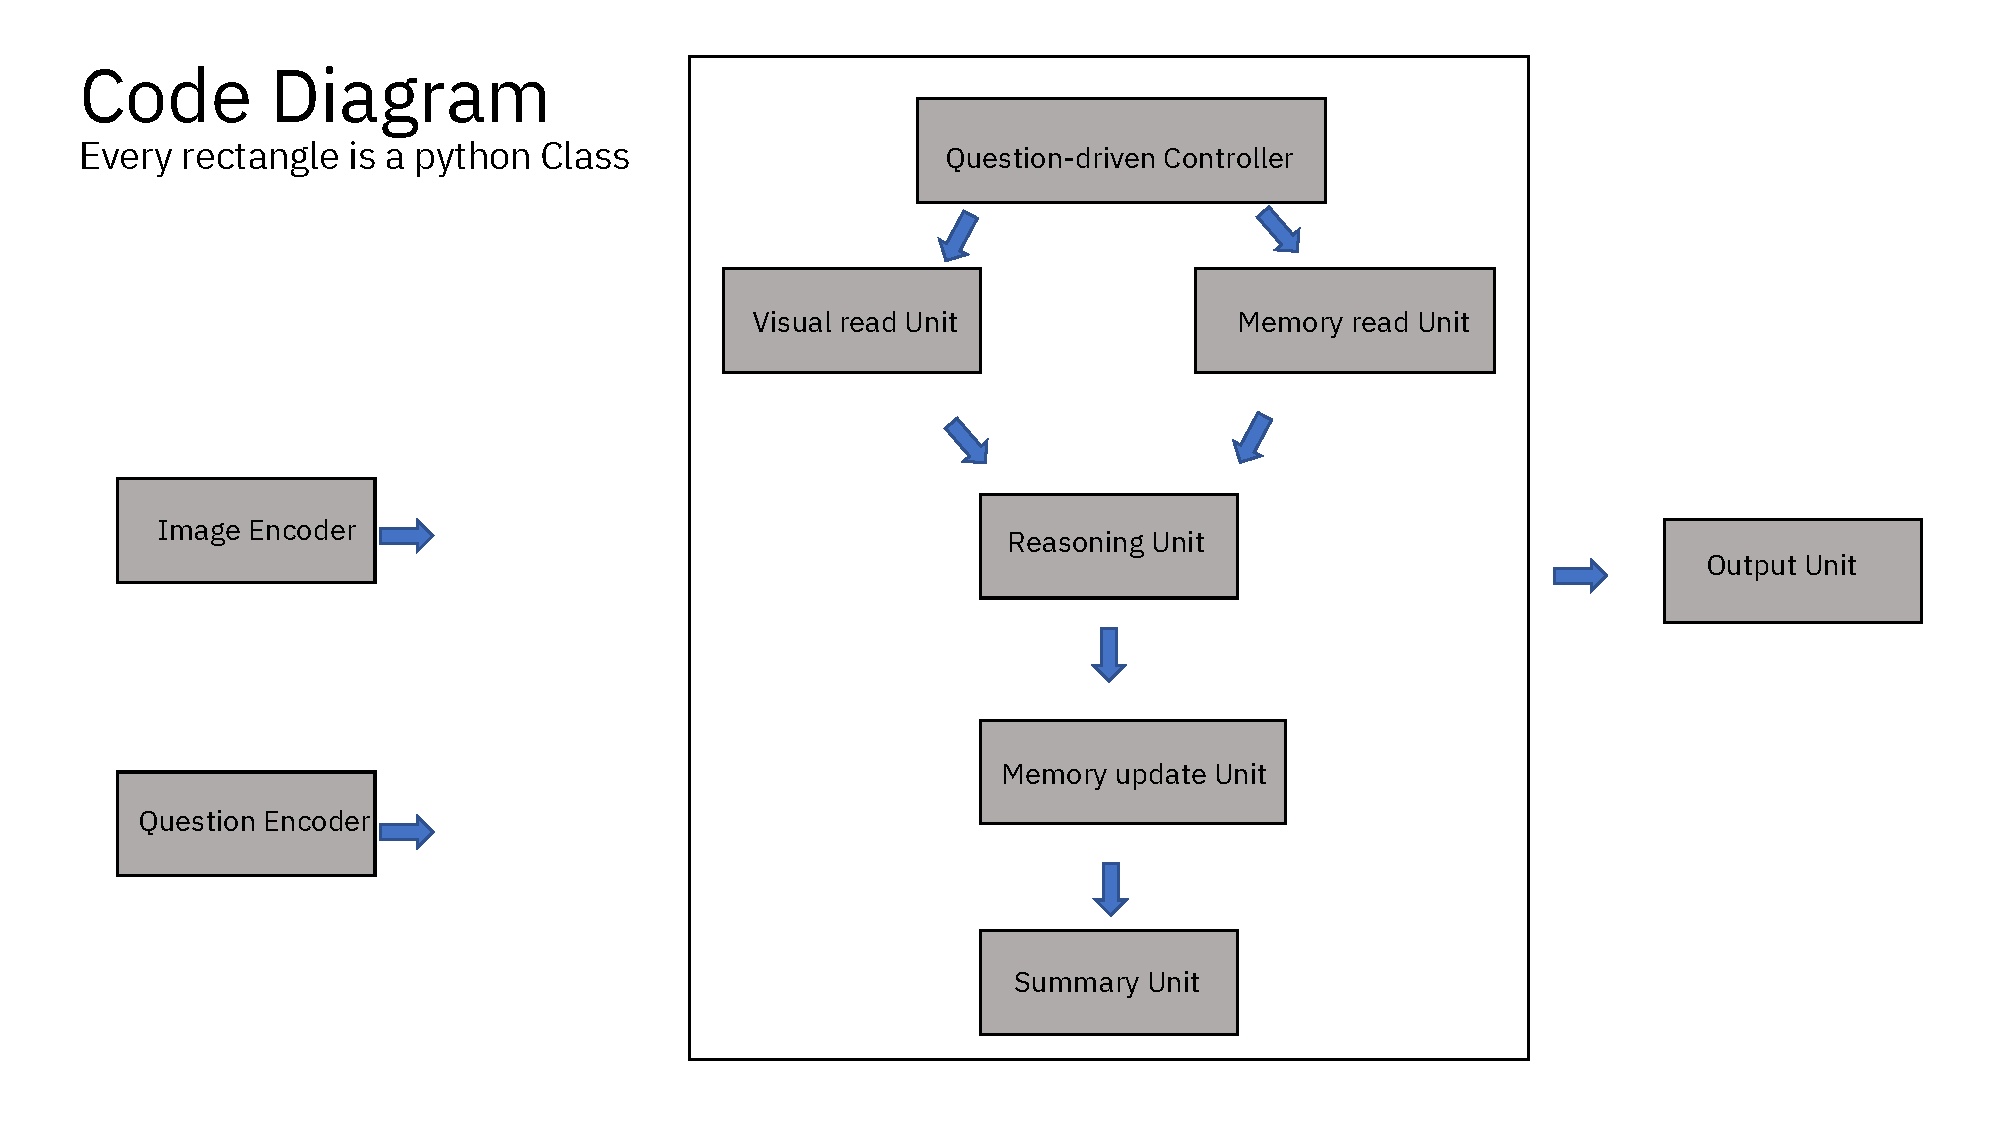
\includegraphics[width=\textwidth]{img/model}
	\caption{Testing}
	\label{fig:model}
\end{figure}


\begin{figure}[ht]
	\centering
	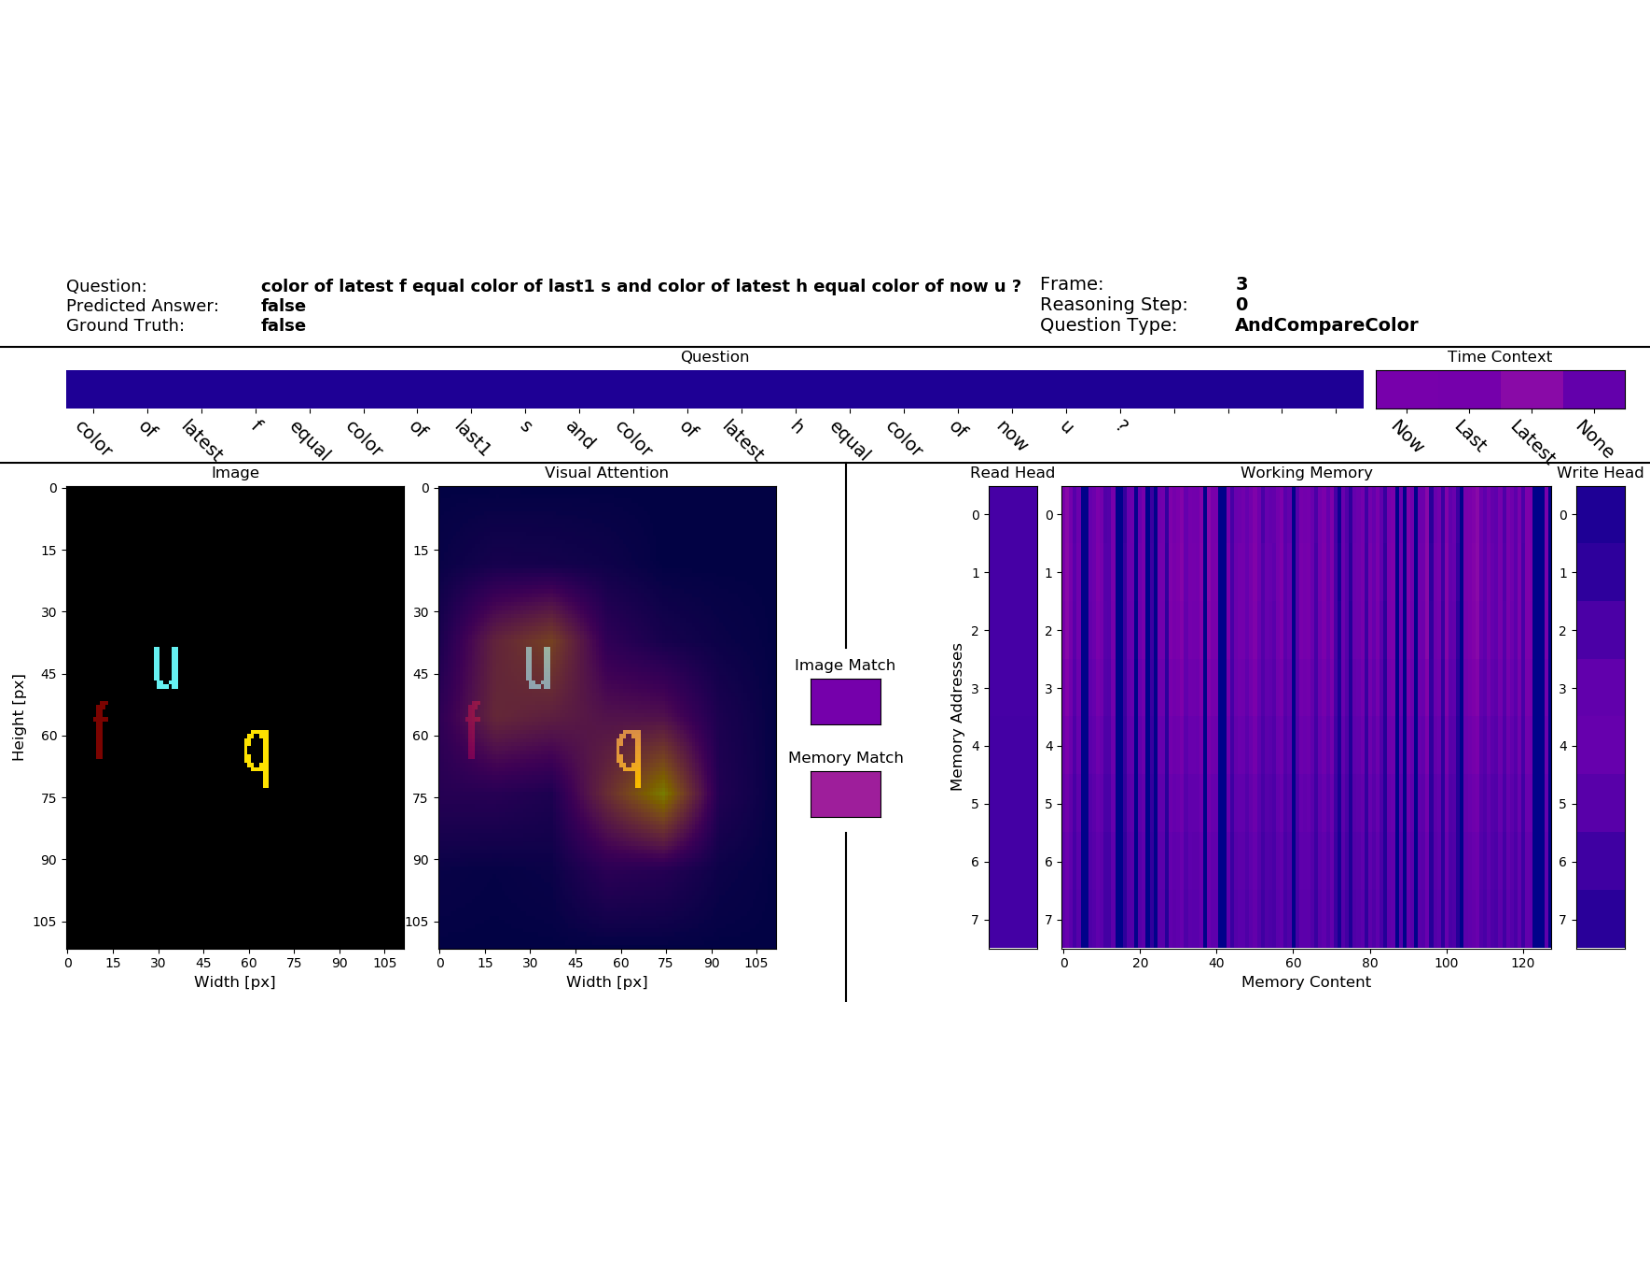
\includegraphics[width=\textwidth]{img/visualization}
	\caption{Testing}
	\label{fig:visualization}
\end{figure}



\newpage
\bibliographystyle{alpha}

\end{document}
